\documentclass{article}
\usepackage[utf8]{inputenc}

\usepackage{amsmath}
\usepackage{hyperref}

\title{ECE342 Final Review - Cramming Carnival}
\author{Author: Members of HKN}
\date{Spring 2024}

\newcommand{\dd}[1]{\mathrm{d}#1}

\usepackage[makeroom]{cancel}
\usepackage[letterpaper, portrait, margin=1in]{geometry}
\usepackage{graphicx}
\usepackage{float}
\usepackage{enumitem}
\usepackage{graphicx}
\usepackage{multicol}

\pagenumbering{arabic}

\begin{document}

\begin{center}
\textbf{
{\Large HKN ECE 342 Final Worksheet - Cramming Carnival}
}
\end{center} 
\noindent\makebox[\linewidth]{\rule{\linewidth}{0.2pt}}
\section*{DC Analysis}
\subsection*{Transistor Parameters}
\textbf{MOSFETs:}
$$\mu_nC_{ox} = 100\:\mu \text{A/V}^2; \ V_{TN} = 1\text{ V}$$
$$\mu_pC_{ox} = 50\:\mu \text{A/V}^2; \ |V_{TP}| = 1\text{ V}$$
\textbf{BJTs:}
$$\beta = 99; V_{\rm BE, on} = 0.7\text{ V}$$
\subsection*{Problem 1}
For this problem, refer to the circuit below. Use $V_{DD} = 5$ V, $I_B = 200\ \mu$A, 1X = $\frac{100}{1}$.
\begin{figure}[!htb]
\begin{center}
    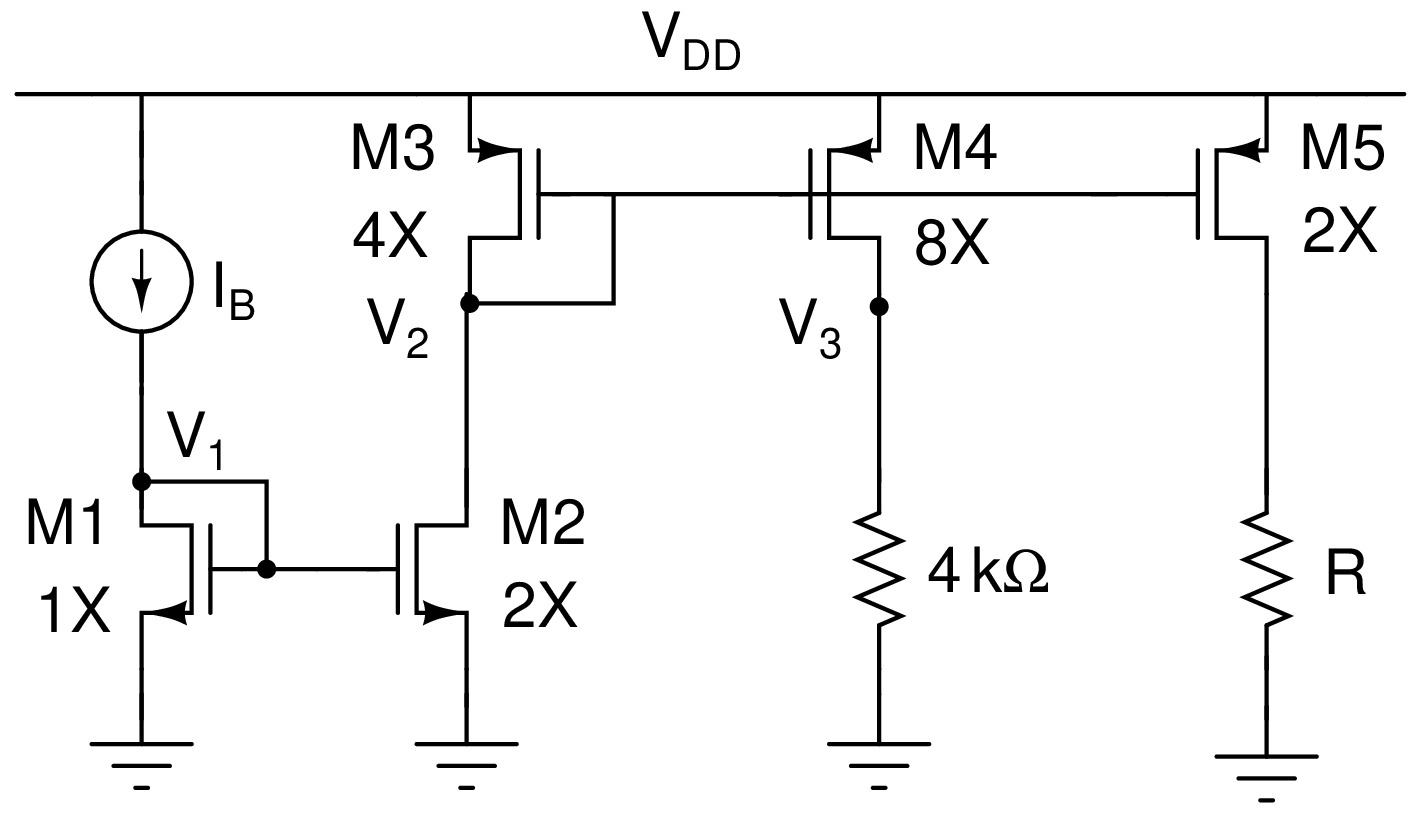
\includegraphics[width=0.7\textwidth]{figures/cc_dc_2 (1).jpg}
\end{center}
\end{figure}
\begin{enumerate}[label=\textbf{(\alph*)}]
    \item Determine the DC voltages $V_1$, $V_2$, and $V_3$.
    \item Determine the value of R such that M5 is biased at the edge of saturation.
\end{enumerate}
\newpage
\subsection*{Problem 2}
For this problem, refer to the circuit below.
\begin{figure}[!htb]
\begin{center}
    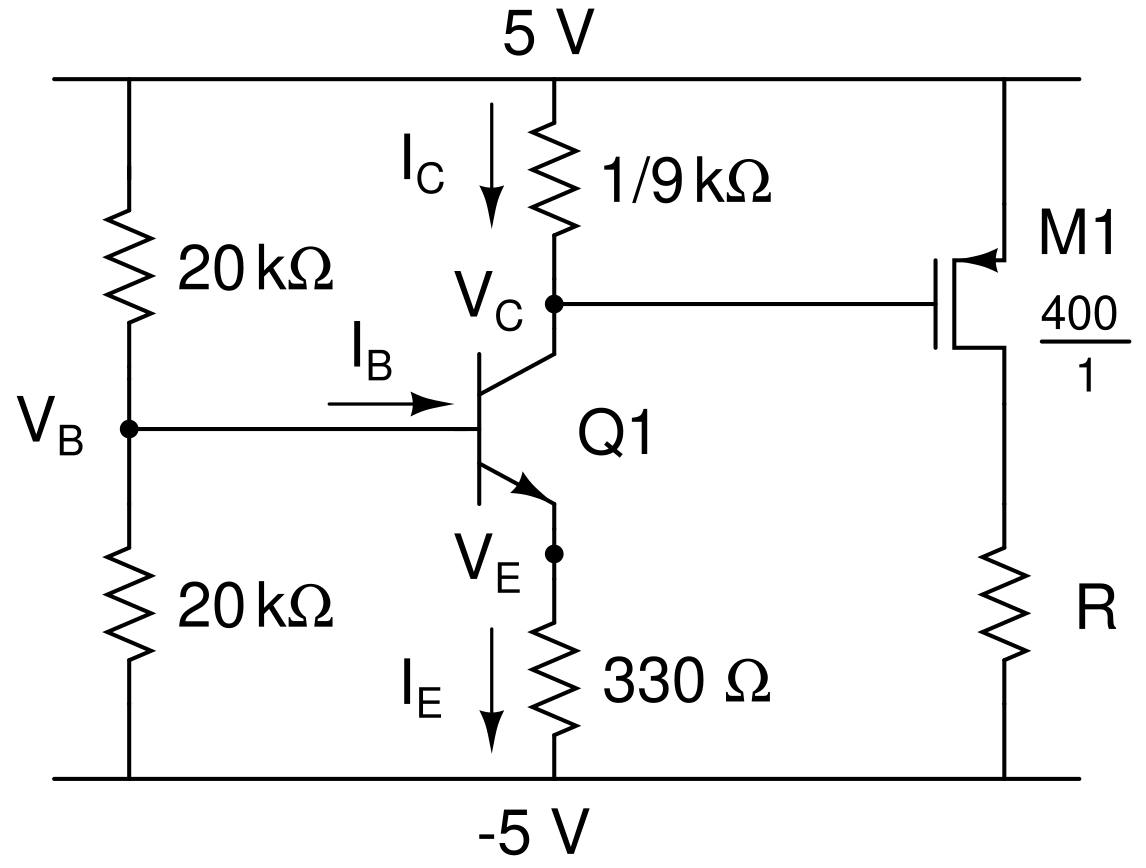
\includegraphics[width=0.6\textwidth]{figures/cc_dc1 (1).png}
\end{center}
\end{figure}
\begin{enumerate}[label=\textbf{(\alph*)}]
    \item Determine the DC currents and voltages $V_B$, $V_E$, $V_C$, $I_B$, $I_E$, and $I_C$ of Q1.  What is its region of operation?
    \item Determine the value of R such that M1 is biased at the edge of saturation.
\end{enumerate}
\newpage
\section*{Small-Signal Analysis}
\subsection*{Problem 1}
Determine the values of $G_M$, $R_{OUT}$, and $A_v = v_{out}/v_{in}$ of this amplifier.  Assume all MOSFETs are biased in saturation.  Do not assume $r_{ds} = \infty$, though you can assume $g_mr_{ds} >> 1$.
\begin{figure}[!h]
\begin{center}
    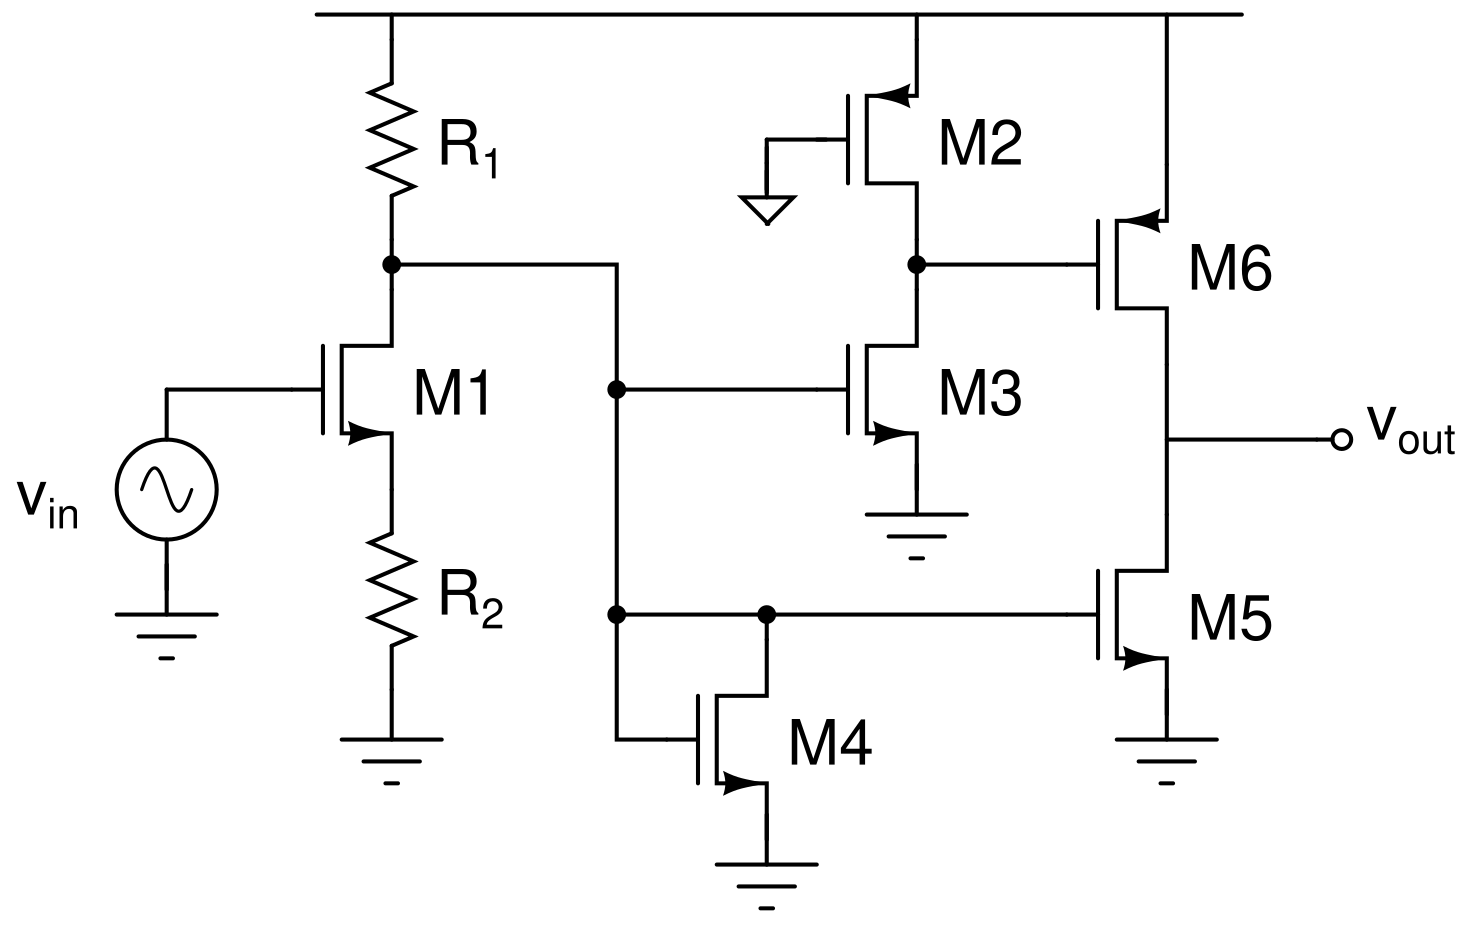
\includegraphics[width=0.85\textwidth]{figures/cc_amp1.png}
\end{center}
\end{figure}
\newpage
\subsection*{Problem 2}
Determine the values of $G_M$, $R_{OUT}$, and $A_v = v_{out}/v_{in}$ of this amplifier.  Assume all MOSFETs are biased in saturation, all BJTs are biased in forward active mode, $r_{ds} \ne \infty$, $r_0 = \infty$, and $g_mr_{ds} \gg 1$.
\begin{figure}[!h]
\begin{center}
    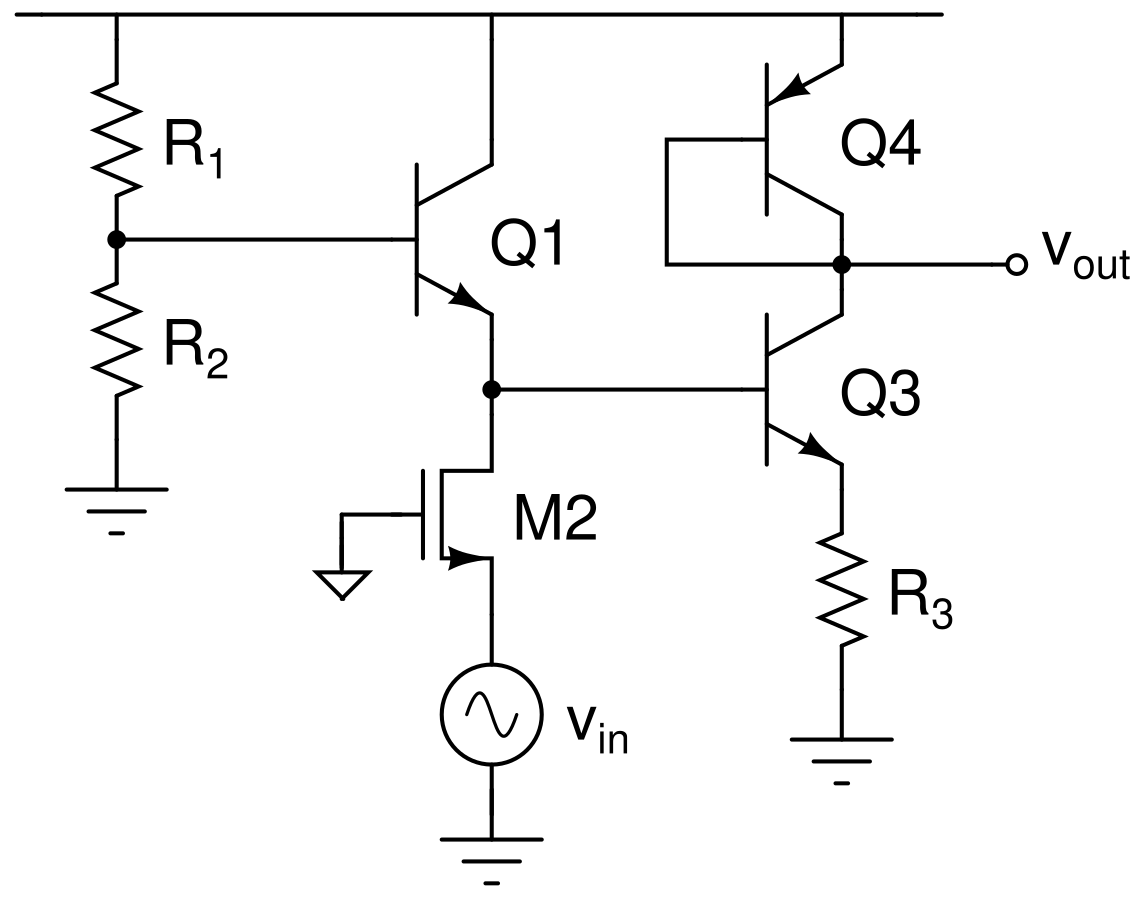
\includegraphics[width=0.65\textwidth]{figures/cc_amp_2.png}
\end{center}
\end{figure}
\newpage
\subsection*{Problem 3}
Determine the values of $G_M$, $R_{OUT}$, and $A_v = v_{out}/v_{in}$ of this amplifier.  Assume all MOSFETs are biased in saturation, all BJTs are biased in forward active mode, $r_{ds} \ne \infty$, $r_0 = \infty$, and $g_mr_{ds} \gg 1$.
\begin{figure}[!h]
\begin{center}
    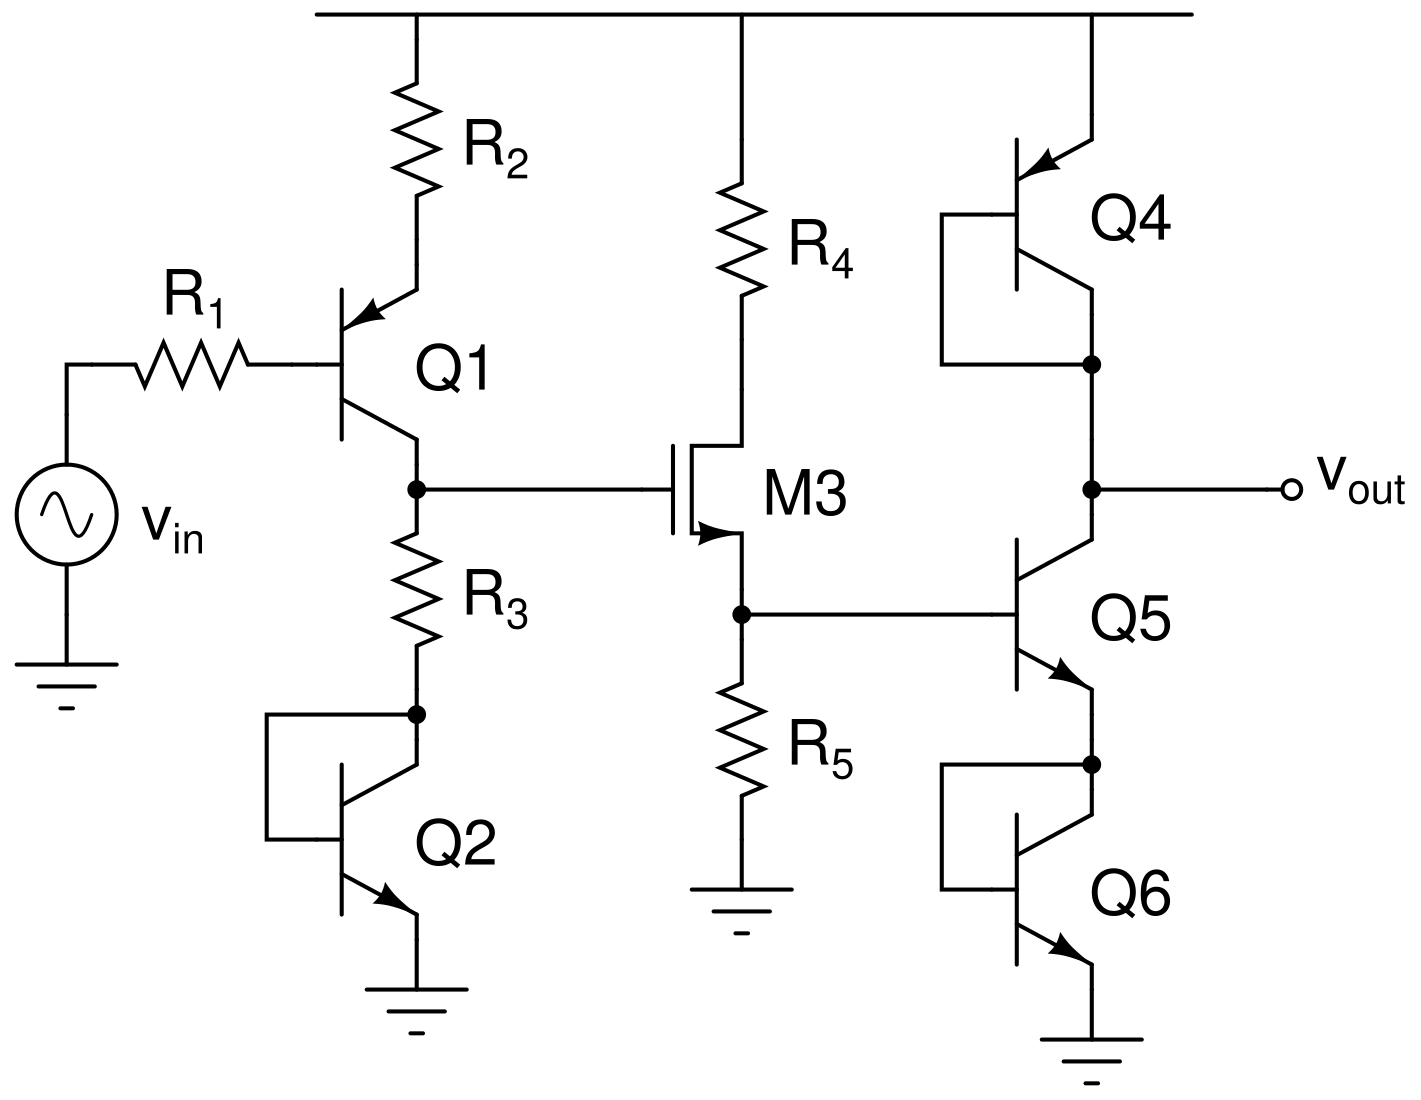
\includegraphics[width=0.75\textwidth]{figures/cc_amp_3.png}
\end{center}
\end{figure}
\newpage
\subsection*{Problem 4}
Determine the values of $G_M$, $R_{OUT}$, and $A_v = v_{out}/v_{in}$ of this amplifier.  Assume all MOSFETs are biased in saturation.  Do not assume $r_{ds} = \infty$, though you can assume $g_mr_{ds} >> 1$.
\begin{figure}[!h]
\begin{center}
    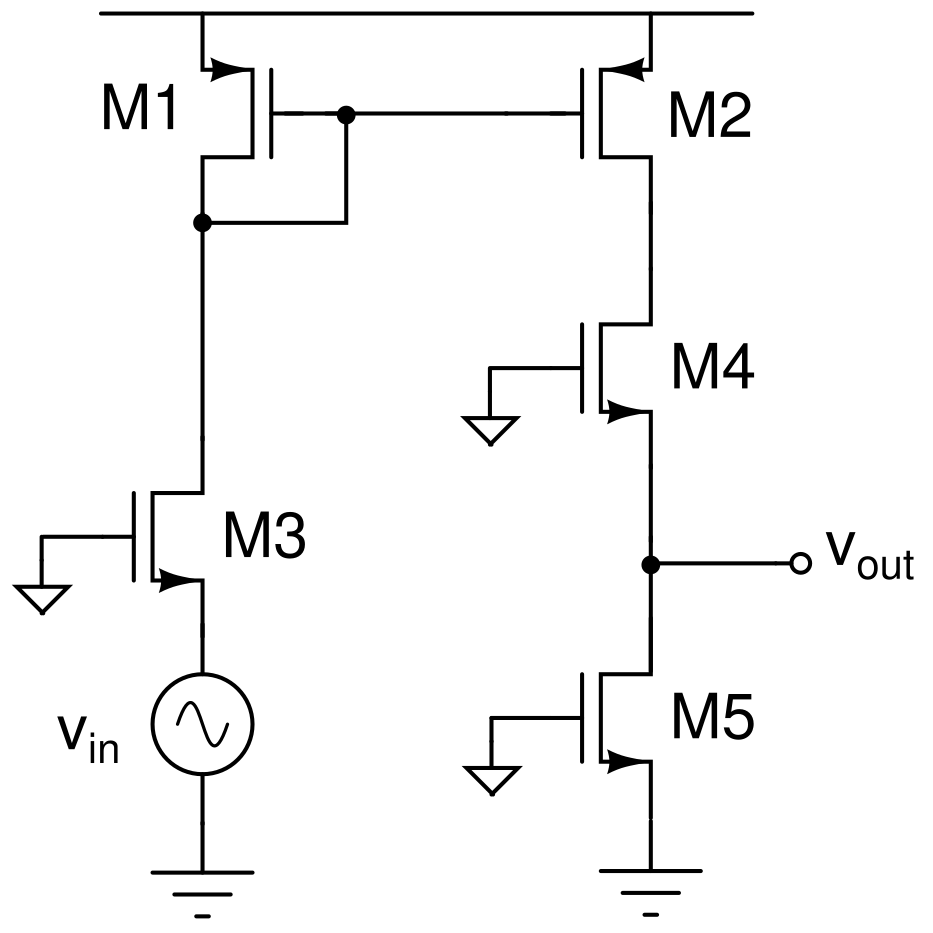
\includegraphics[width=0.5\textwidth]{figures/cc_amp_4.png}
\end{center}
\end{figure}
\newpage
\subsection*{Problem 5}
Determine the values of $G_M$, $R_{OUT}$, and $A_v = v_{out}/v_{in}$ of this amplifier.  Assume all MOSFETs are biased in saturation, all BJTs are biased in forward active mode, $r_{ds} \ne \infty$, $r_0 = \infty$, and $g_mr_{ds} \gg 1$. 
\begin{figure}[!h]
\begin{center}
    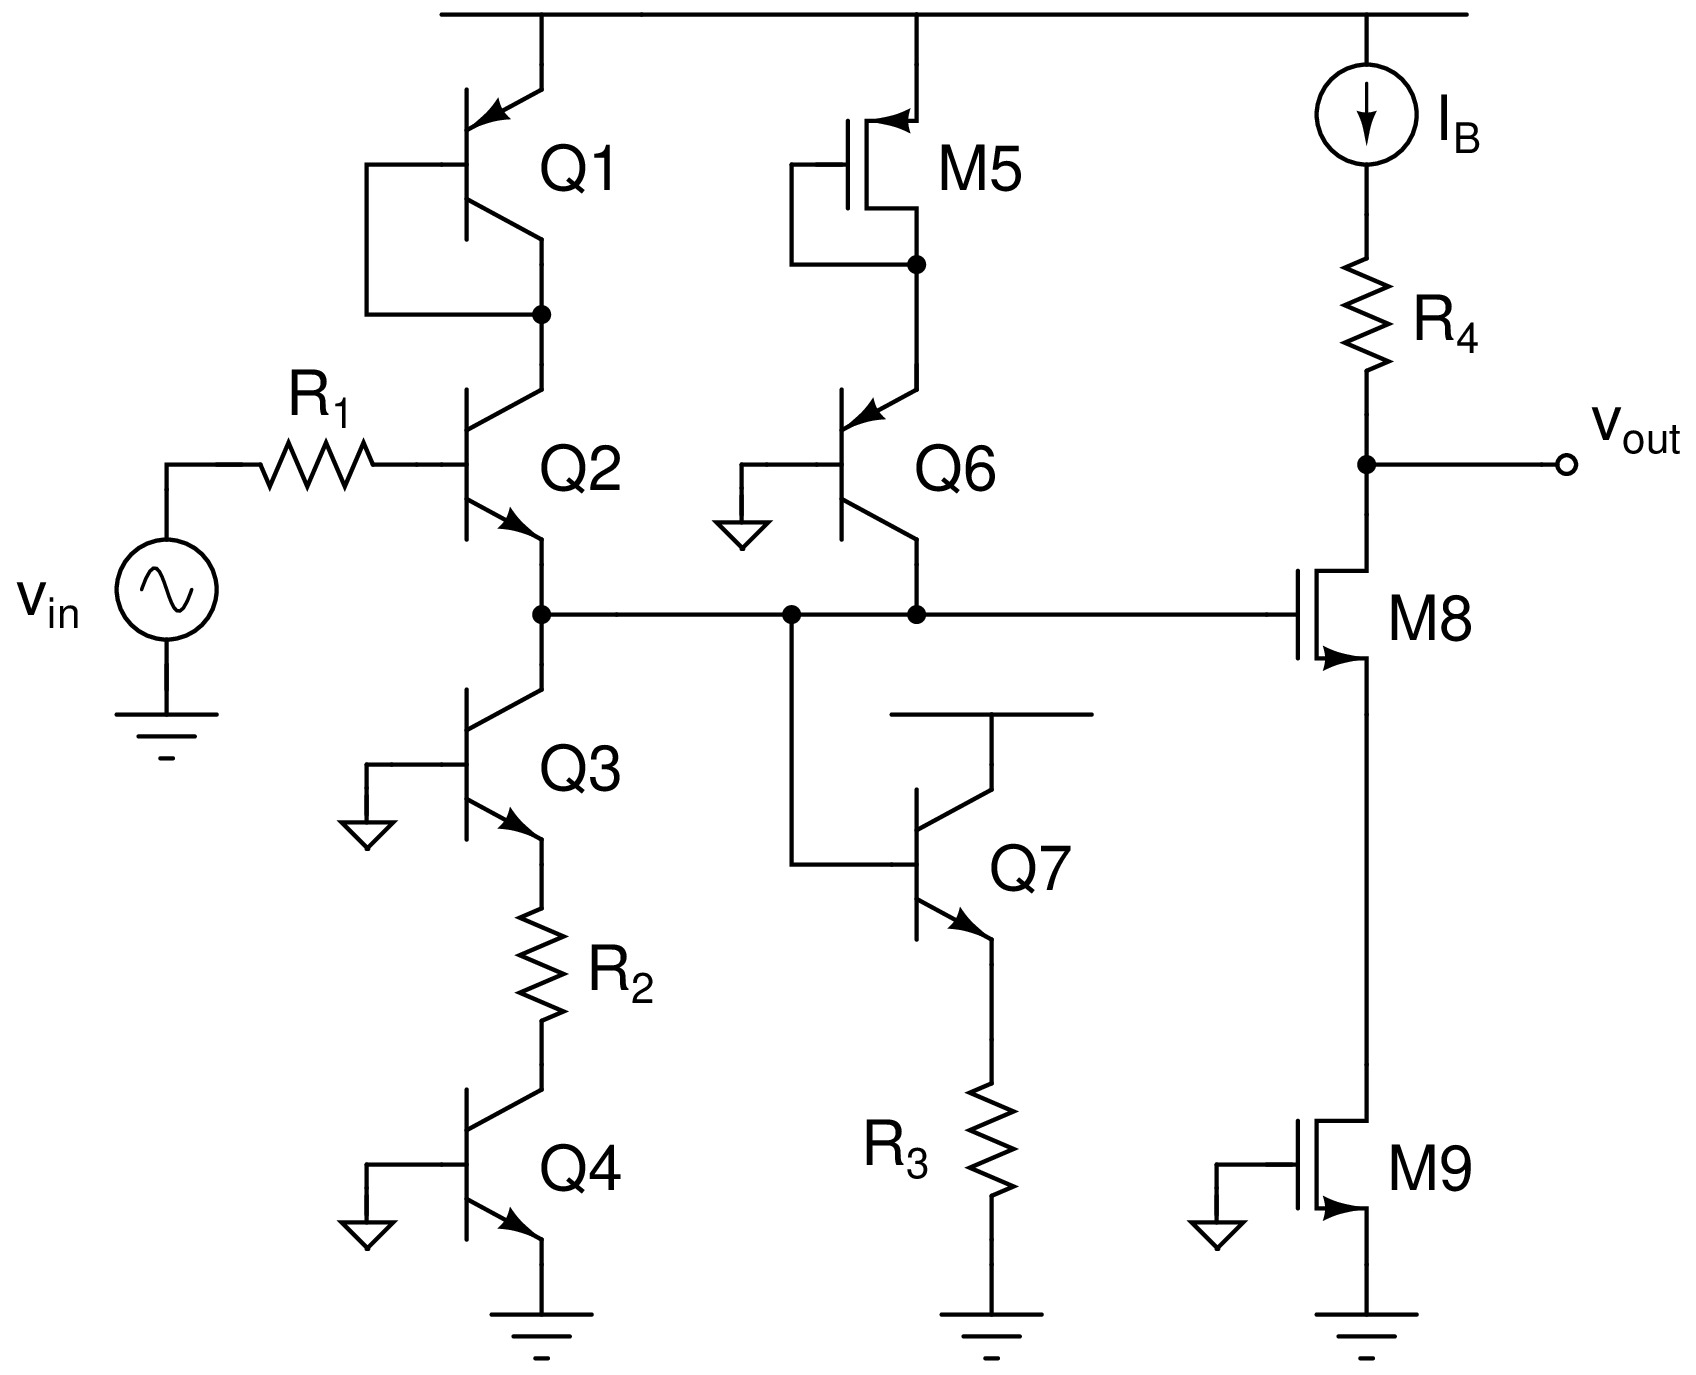
\includegraphics[width=0.8\textwidth]{figures/cc_amp5.jpg}
\end{center}
\end{figure}
\newpage
\section*{Bode Plots}
\subsection*{Problem 1}
For the following amplifier transfer functions, \textbf{(i)} plot the magnitude response, \textbf{(ii)} determine the unity gain frequency, and \textbf{(iii)} plot the phase response:
\begin{enumerate}[label=\textbf{(\alph*)}]
    \item $$H(s) = \frac{10^4}{s(1+s/10^3)}$$
    \item $$H(s) = \frac{2000\left(1 + s/10^2\right)}{\left(1 + s/10\right)\left(1 + s/10^3\right)\left(1 + s/10^4\right)}$$
    \item $$H(s) = \frac{4000(1+s/10^2)}{(1+s/10)(1+s/10^4)^2}$$
\end{enumerate}
\newpage
\subsection*{Problem 2}
For each of the amplifier transfer functions in Problem 1, determine the incremental output voltage response $v_{out}(t)$ to an incremental input voltage $v_{in}(t) = 10\cos(10^3 \cdot t)$ mV.
\newpage
\section*{Open Circuit Time Constants}
\subsection*{Problem 1}
Use the open-circuit time constant method to estimate the -3 dB frequency, $\omega_{\rm -3 dB}$, of this amplifier.  Consider $C_{gs}$, $C_{gd}$, $C_{\pi}$, $C_{\mu}$, and $r_{ds}$.  Ignore $r_0$. \\ 
\begin{figure}[!h]
\begin{center}
    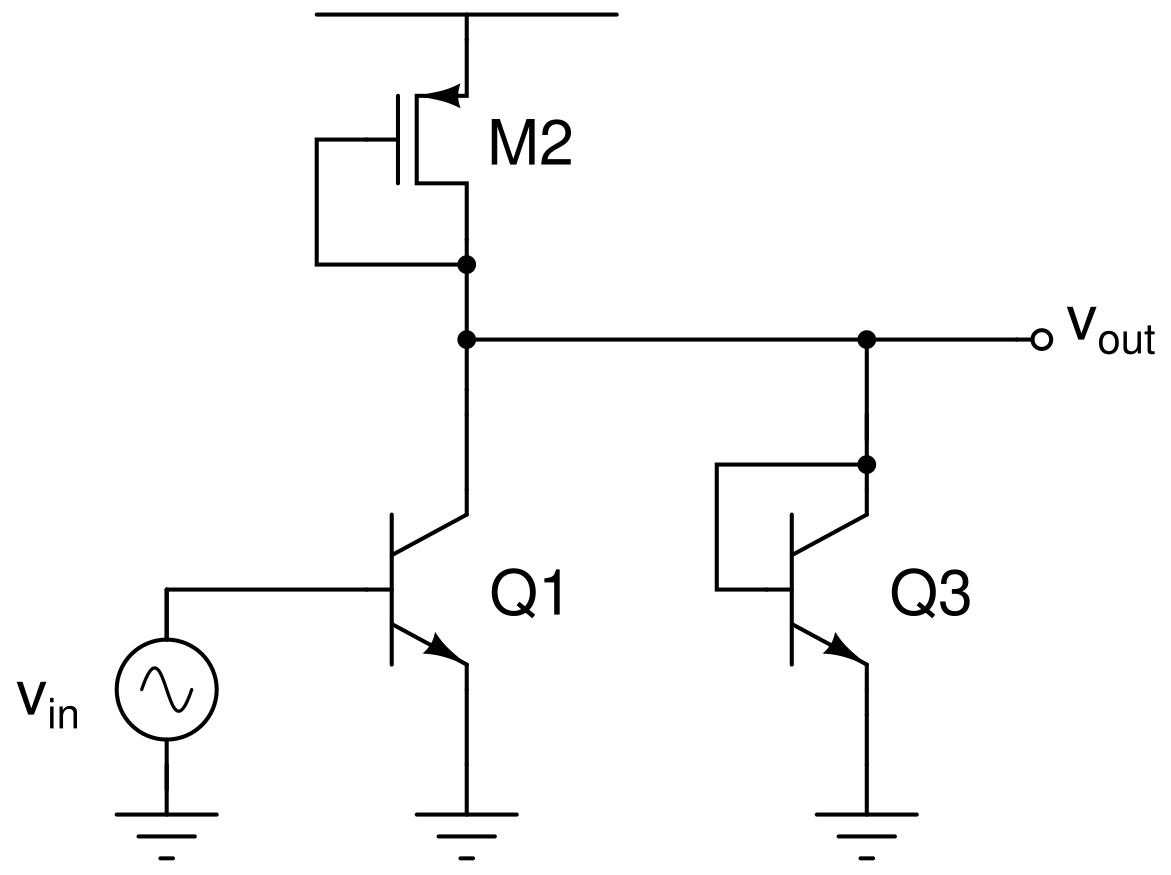
\includegraphics[width=0.65\textwidth]{figures/cc_octc2.png}
\end{center}
\end{figure}
\newpage
\subsection*{Problem 2}
Use the open-circuit time constant method to estimate the -3 dB frequency, $\omega_{\rm -3 dB}$, of this amplifier.  Consider $C_{gs}$, $C_{gd}$, $C_{\pi}$, $C_{\mu}$, and $r_{ds}$.  Ignore $r_0$. \\ 
\begin{figure}[!h]
\begin{center}
    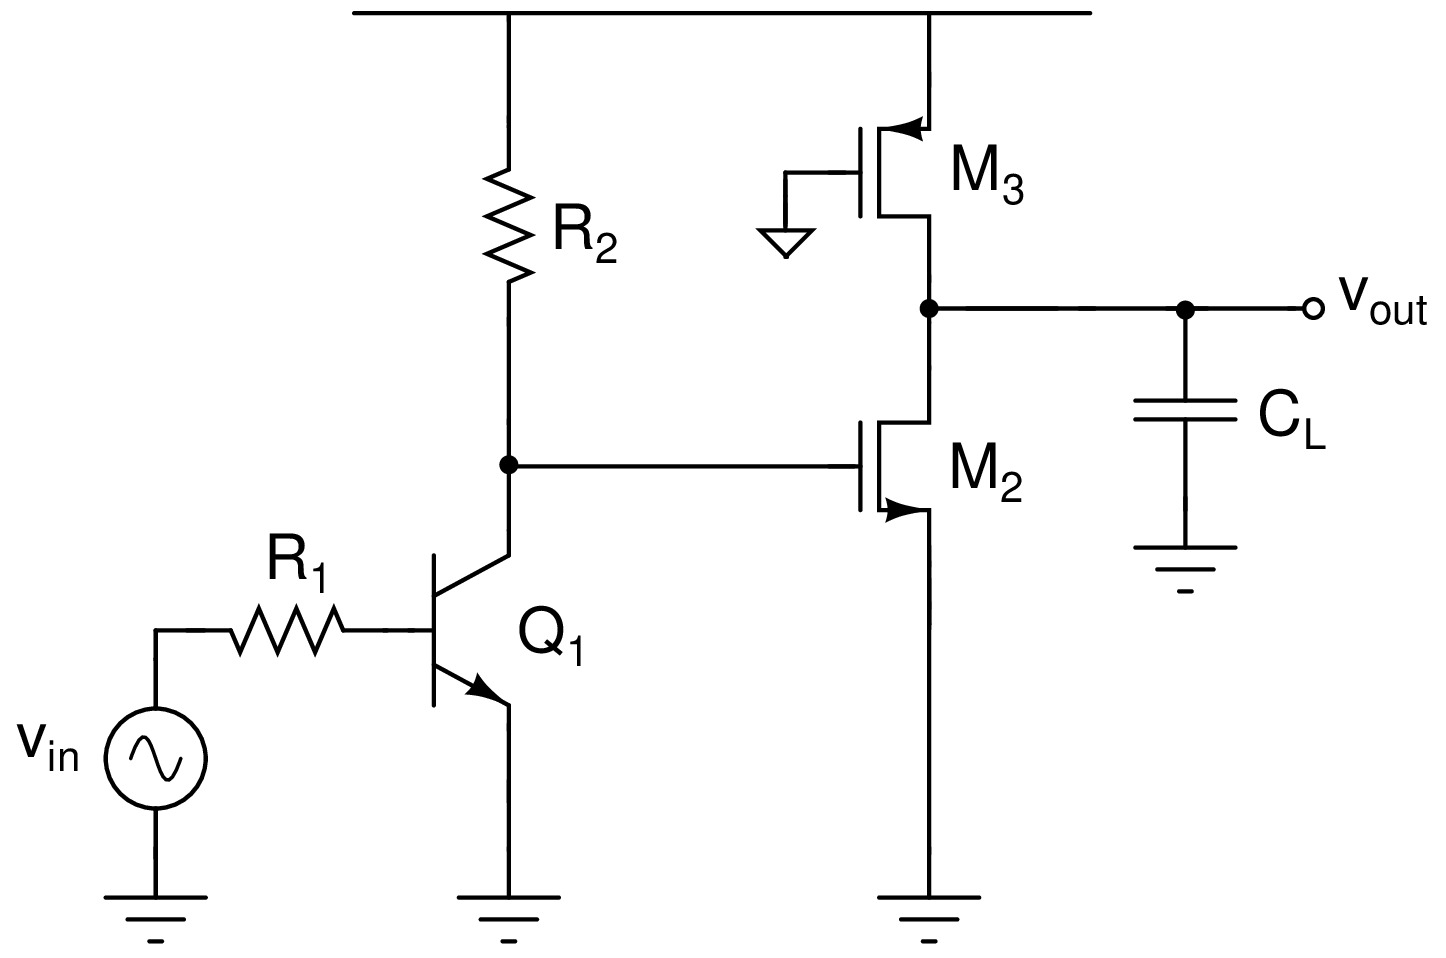
\includegraphics[width=0.7\textwidth]{figures/cc_octc1.jpg}
\end{center}
\end{figure}
\newpage
\subsection*{Problem 3}
Use the open-circuit time constant method to estimate the -3 dB frequency, $\omega_{\rm -3 dB}$, of this amplifier.  Consider $C_{gs}$, $C_{gd}$, $C_{\pi}$, $C_{\mu}$, and $r_{ds}$. 
\begin{figure}[!h]
\begin{center}
    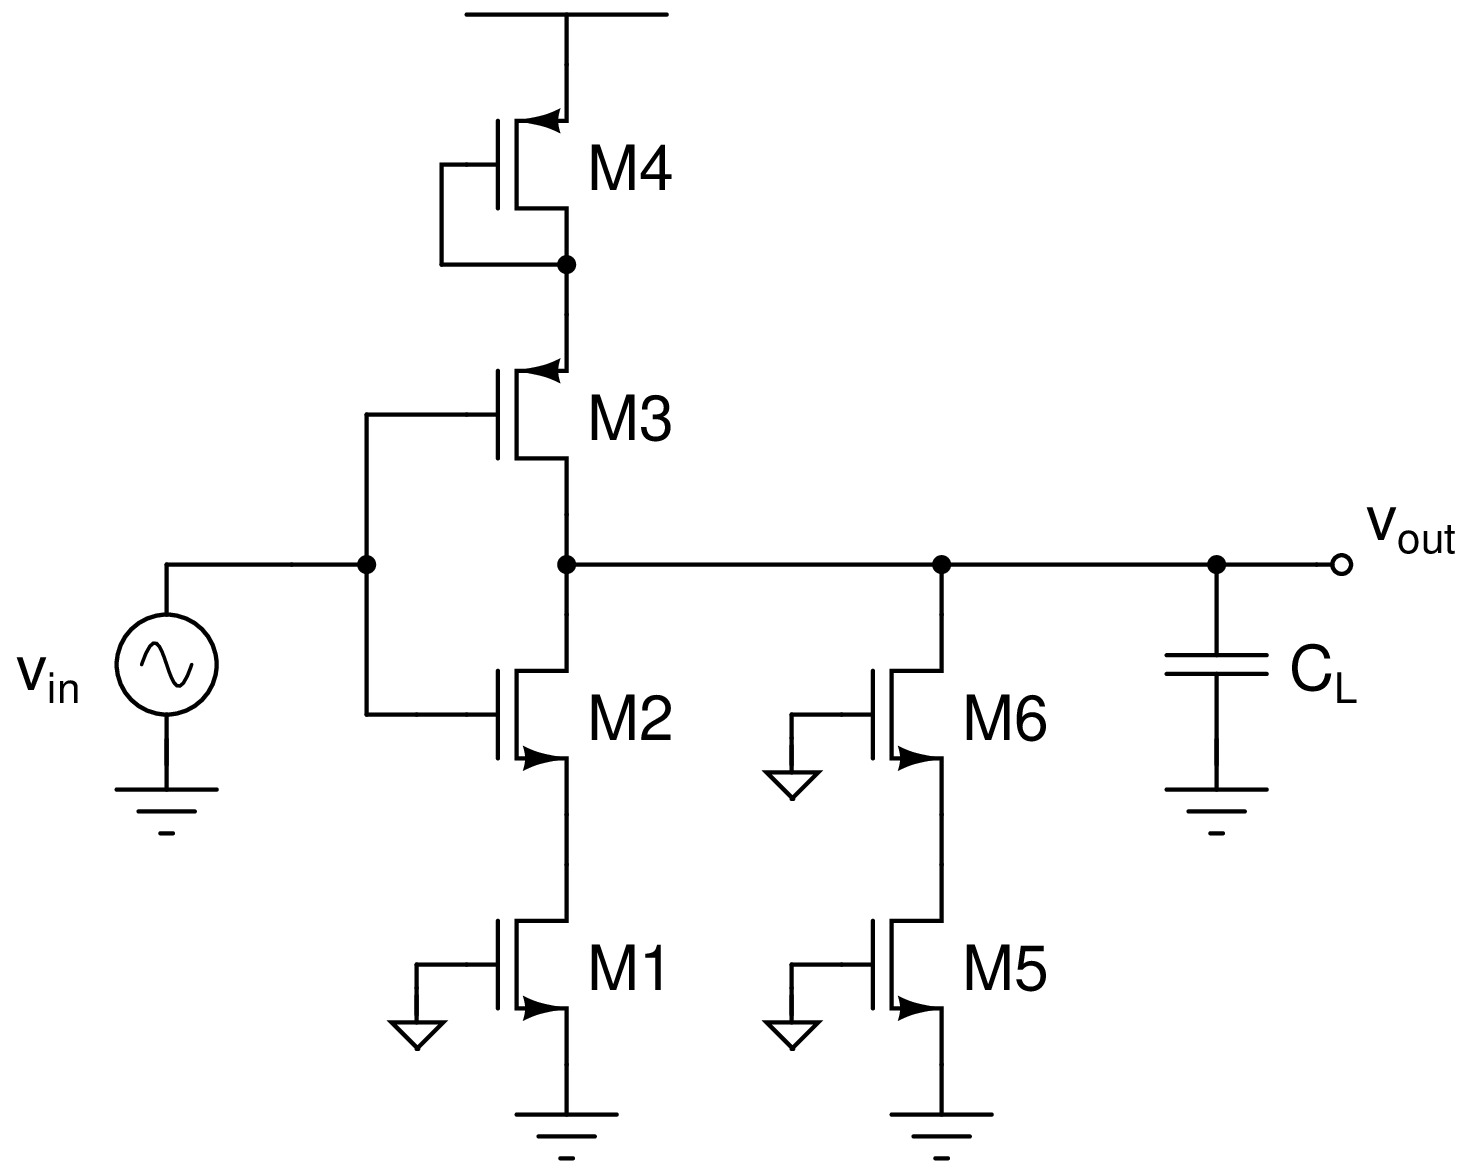
\includegraphics[width=0.7\textwidth]{figures/cc_octc3 (2).jpg}

\end{center}
\end{figure}
\newpage
\section*{CMOS Logic Circuits}
For each part, design and draw the schematic of a CMOS logic gate that implements the Boolean expression. In each schematic, label the size of each transistor such that the worst case delays of the pull-up and pull-down networks are equivalent to those of a standard minimum-sized inverter with $(W/L)_P/(W/L)_N$ = 2.  Inverted inputs are not available.
\begin{enumerate}[label=(\alph*)]
    \item $Z_1 = \overline{(A+B) \cdot C}$
    \item $Z_2 = \overline{(A \cdot B \cdot C) + (D \cdot E)}$
    \item $Z_3 = \overline{A} \cdot (\overline{B} + \overline{C} + \overline{D})$
\end{enumerate}
\newpage

\end{document}